\documentclass[10pt]{article}
\usepackage[utf8]{inputenc}
% \usepackage{fullpage}
\usepackage[left=2.5cm,right=2.5cm,top=2.5cm,bottom=2.5cm,a4paper]{geometry}
\usepackage[onehalfspacing]{setspace}
\usepackage{graphicx,float,subcaption,multirow}
\DeclareGraphicsExtensions{.pdf,.png,.jpg,.jpeg}
\usepackage{kotex}
\usepackage{amsmath, amsfonts, amssymb, amsthm}
\usepackage{textcomp}
\usepackage{physics, mhchem}
\usepackage{xcolor}
% \setlength\parindent{0pt}
\usepackage{indentfirst}
\usepackage[shortlabels]{enumitem}
\usepackage{listings}
\usepackage{multicol}

\definecolor{codegreen}{rgb}{0,0.6,0}
\definecolor{codeblue}{RGB}{26,26,255}
\definecolor{codegray}{rgb}{0.5,0.5,0.5}
\definecolor{codepurple}{rgb}{0.58,0,0.82}
\definecolor{backcolour}{rgb}{0.95,0.95,0.92}

\lstdefinestyle{mystyle}{
    backgroundcolor=\color{backcolour},   
    commentstyle=\color{codegreen},
    keywordstyle=\color{magenta},
    numberstyle=\tiny\color{codegray},
    stringstyle=\color{codepurple},
    basicstyle=\ttfamily\footnotesize,
    breakatwhitespace=false,         
    breaklines=true,                 
    captionpos=b,                    
    keepspaces=true,                 
    numbers=left,                    
    numbersep=1pt,                  
    showspaces=false,                
    showstringspaces=false,
    showtabs=false,                  
    tabsize=4,
    columns=fullflexible,
    escapeinside={<@}{@>}
}
\lstset{style=mystyle}

\begin{document}
    \begin{center}
        {\LARGE Logic Design Final Project} \\
        \vspace{2mm}
        공과대학 컴퓨터공학부 \\
        2021-16988 박재완
    \end{center}
    
    \section{Structure}
    \begin{figure}[H]
        \centering
        \includegraphics[width=0.99\textwidth]{../images/diagram.jpg}
        \caption{\small 구현한 microprocessor의 구조}
    \end{figure}
    위와 같은 구조를 갖는 microprocessor를 Verilog와 FPGA 보드를 이용하여 구현하였다.
    전체를 구성하는 각 단위(Adder, MUX, Control Unit, Register, ALU, Data Memory, Program Counter)를 Verilog 모듈로 하나씩 정의하였고, 하나의 파일에서 이들을 전부 wire로 연결하여 정해진 작업을 수행할 수 있도록 하였다.
    Microprocessor가 하는 역할은, 외부로부터 받은 8bit instruction을 해석하여 명령에 따라 register 및 data memory를 변화시키고, 지정된 output을 7 segment display에 출력하는 것이었다.
    Instruction의 해석은 주어진 과제 스펙을 따랐다.

    \section{Components}
    
    \subsection{Register}
    \begin{lstlisting}[language=Verilog, caption=register\_module.v]
`timescale 1ns / 1ps

module register_module(
    input [1:0] read_register_one,
	input [1:0] read_register_two,
	input [1:0] write_register,
	input [7:0] write_data,
	input RegWrite,
	input CLK,
	input reset,
	output [7:0] read_data_one,
	output [7:0] read_data_two
	);
	
	reg [7:0] registers [0:3];
	
	integer i;
	initial begin
	for (i = 0; i < 4; i = i + 1)
		registers[i] <= 0;
	end
	
	assign read_data_one = registers[read_register_one];
	assign read_data_two = registers[read_register_two];
	
	always @(posedge CLK or posedge reset) begin
        if (reset) begin
            for (i = 0; i < 4; i = i + 1)
                registers[i] <= 0;
        end else begin
            if (RegWrite)
                registers[write_register] <= write_data;
        end
    end

endmodule
    \end{lstlisting}

    7bit 데이터를 저장하고, 읽거나 수정이 가능한 register 모듈을 만들었다. 
    과제 스펙에 따라 총 4개의 레지스터를 안에 두었으며, 전부 0으로 초기화한 뒤 입력 명령에 따라 동작을 수행하도록 하였다.
    `read\_register\_one'과 `read\_register\_two'로 읽어올 레지스터 인덱스를 받으면 각각에 저장된 값을 `read\_data\_one', `read\_data\_two'로 출력하였다.
    또한 RegWrite 신호가 들어올 경우 `write\_register' 인덱스의 레지스터에 `write\_data' 값을 저장하였다. 
    이때 레지스터 값 변경은 입력되는 clock 신호에 positive edge triggered 되도록 always 문으로 설정해주었다.
    또한 reset이 입력된 경우는 clock과 무관하게 모든 레지스터의 값을 0으로 초기화해주었다.

    \subsection{Control Unit}
    \begin{lstlisting}[language=Verilog, caption=control\_unit.v]
`timescale 1ns / 1ps

module control_unit(
	input [1:0] op,
	output RegDst,
	output RegWrite,
	output ALUSrc,
	output Branch,
	output MemRead,
	output MemWrite,
	output MemtoReg,
	output ALUOp
    );
	 
	reg [7:0] out;
	assign {RegDst, RegWrite, ALUSrc, Branch, MemRead, MemWrite, MemtoReg, ALUOp} = out;
	
	always @(op) begin
        case (op)
            0: out = 8'b11000001;
            1: out = 8'b01101010;
            2: out = 8'b00100100;
            3: out = 8'b00010000;
        endcase
    end

endmodule
    \end{lstlisting}

    Instruction의 최상위 두 비트에는 microprocessor가 수행할 작업의 종류가 나타나있는데, control unit은 이를 받아 다른 모듈들에 어떤 동작을 수행할지 알려주는 신호를 출려한다.
    과제 스펙에 맞게 4가지 입력에 따라 RegDst, RegWrite, ALUSrc, Branch, MemRead, MemWrite, MemtoReg, ALUOp의 값을 정해주었다.

    \subsection{ALU}
    \begin{lstlisting}[language=Verilog, caption=ALU.v]
`timescale 1ns / 1ps

module ALU(
    input signed [7:0] A,
	input signed [7:0] B,
	input ALUOp,
	output signed [7:0] O
	);
	
	assign O = ALUOp ? A + B : A + B;

endmodule
    \end{lstlisting}

    `ALUOp' 신호에 따라 두 가지 동작을 수행하는 ALU를 구현하였다. 다만 본 과제에서는 이 신호와 무관하게 ALU가 언제나 덧셈만을 구현하여야 했기 때문에, `ALUOp' 값과 무관하게 결과를 출력하였다.
    또한 본 과제에서는 overflow가 발생하는 상황은 배제하였기 때문에 carry-out은 신경쓰지 않았다.
    
    \subsection{Data Memory}
    \begin{lstlisting}[language=Verilog, caption=data\_memory.v]
`timescale 1ns / 1ps

module data_memory(
	input [7:0] address,
	input [7:0] write_data,
	input MemWrite, MemRead,
	input CLK,
	input reset,
	output reg [7:0] read_data
	);

	reg [7:0] MEMORY [0:31];

	integer i;
	initial begin
		for (i=0; i<32; i=i+1)
			MEMORY[i] = i < 16 ? i : 16 - i;
	end

	always @(posedge CLK or posedge reset) begin
        if (reset) begin
            for (i=0; i<32; i=i+1)
                MEMORY[i] <= i < 16 ? i : 16 - i;
        end else begin
            if (MemWrite == 1) begin
                MEMORY[address] <= write_data;
            end
        end
    end
		
	always @(address or MemRead) begin
        if (MemRead == 1)
            read_data <= MEMORY[address];
    end

endmodule
    \end{lstlisting}

    7bit 데이터를 저장하는 메모리를 구현하였다. 
    총 32개의 데이터를 저장하였고, 순서대로 `0, 1, $\cdots$, 15, 0, -1, $\cdots$, -15'로 초기화해주었다.
    또한 이 역시 특정 위치의 데이터를 읽어 출력하거나, 데이터를 수정하는 동작을 할 수 있도록 하였다.
    `MemRead' 신호가 들어온 경우 `address'의 값을 `read\_data'에 출력하였고, `MemWrite' 신호가 들어온 경우 `address' 위치의 데이터를 `write\_data'로 바꿔주었다.
    또한 값의 수정은 clock 신호에 positive edge triggered 되도록 always 문으로 설정해주었다.
    나머지 reset이나 값 출력 동작은 clock과 무관하게 동작하도록 하였다.
    
    \subsection{Program Counter}
    \begin{lstlisting}[language=Verilog, caption=PC.v]
`timescale 1ns / 1ps

module PC(
    input CLK,
	input reset,
	input [7:0] D,
	output reg [7:0] Q
	);
	
	initial Q = 0;
	
	always @(posedge CLK or posedge reset) begin
        if (reset)
            Q <= 0;
        else
            Q <= D;
    end

endmodule
    \end{lstlisting}
    외부로부터 받아오는 instruction의 address를 바꾸어주는 역할을 한다.
    기본적으로 `D'에 들어온 값으로 `Q'를 바꾸어주고, core logic에 있는 combinational circuit을 거쳐 `D' 값이 결정되어 들어오면 다음 address가 결정된다.

    \subsection{MUX}
    \begin{multicols}{2}
    \begin{lstlisting}[language=Verilog, caption=MUX\_two.v]
`timescale 1ns / 1ps

module MUX_two(
    input [1:0] I0,
	input [1:0] I1,
	input S0,
	output [1:0] Z
	);
	
	assign Z = S0 ? I1 : I0;

endmodule
    \end{lstlisting}
    \begin{lstlisting}[language=Verilog, caption=MUX\_eight.v]
`timescale 1ns / 1ps

module MUX_eight(
    input [7:0] I0,
	input [7:0] I1,
	input S0,
	output [7:0] Z
	);
	
	assign Z = S0 ? I1 : I0;

endmodule
    \end{lstlisting}
    \end{multicols}

    입력된 control input (`S0')에 따라 두 값 중 하나를 선택해주는 2 to 1 MUX를 구현하였다.
    실제 logic에서는 2bit, 8bit의 두 가지로 사용해야했기에 두 개의 모듈을 만들어주었다.
    
    \subsection{Frequency Divider}
    \begin{lstlisting}[language=Verilog, caption=frequency\_divider.v]
`timescale 1ns / 1ps

module frequency_divider(
    input clkin,
    input clr,
    output reg clkout
    );
	 
	reg [31:0] cnt;
	initial begin
        cnt = 0;
        clkout = 0;
	end
	
	always @(posedge clkin or posedge clr) begin
        if(clr) begin
            cnt <= 32'd0;
            clkout <= 1'b0;
        end else if(cnt == 32'd25000000) begin
            cnt <= 32'd0;
            clkout <= ~clkout;
        end else begin
            cnt <= cnt + 1;
        end
    end

endmodule
    \end{lstlisting}

    사용할 보드의 clock은 50MHz 신호를 주었는데, 과제 스펙에서는 1초에 한번 결과가 바뀌기를 요구했기에 진동수를 나누어주는 모듈을 제작하였다.
    Clock이 25000000번의 주기동안 움직일때마다 출력 clock을 toggle 시켜 결과적으로 50MHz 신호를 1Hz 신호로 변환할 수 있도록 하였다.
    
    \subsection{7 Segment Hexadecimal Decoder}
    \begin{lstlisting}[language=Verilog, caption=hex\_to\_7.v]
`timescale 1ns / 1ps

module hex_to_7(
    input [3:0] hex,
    output reg [6:0] seg
    );

	always @(hex) begin
        case (hex)
            0: seg <= 7'b0111111;
            1: seg <= 7'b0000110;
            2: seg <= 7'b1011011;
            3: seg <= 7'b1001111;
            4: seg <= 7'b1100110;
            5: seg <= 7'b1101101;
            6: seg <= 7'b1111101;
            7: seg <= 7'b0000111;
            8: seg <= 7'b1111111;
            9: seg <= 7'b1101111;
            10:seg <= 7'b1110111;
            11:seg <= 7'b1111100;
            12:seg <= 7'b0111001;
            13:seg <= 7'b1011110;
            14:seg <= 7'b1111001;
            15:seg <= 7'b1110001;
        endcase
    end

endmodule
    \end{lstlisting}

    4bit binary input을 16진수로 변환하여 0 - F를 7 segment display의 7bit pattern으로 출력해주는 모듈을 만들었다.

    \section{Core Logic}
    \begin{lstlisting}[language=Verilog, caption=microprocessor.v]
`timescale 1ns / 1ps

module microprocessor(
	input CLKin,
	input reset,
	input [7:0] instruction,
	output [7:0] read_address,
	output [6:0] seg_h,
	output [6:0] seg_l
	);

	wire [1:0] op, rs, rt, rd;
	wire [7:0] sign_extended_rd;
	wire [1:0] write_register;
	wire [7:0] reg_write_data, read_data_one, read_data_two;
	wire [7:0] ALU_second_input, ALU_output;
	wire [7:0] read_data_memory;
	wire [7:0] PC_in;
	wire [7:0] PC_out;
	wire [7:0] MUX_0, MUX_1;
	wire CLK;
	wire RegDst, RegWrite, ALUSrc, Branch, MemRead, MemWrite, MemtoReg, ALUOp;
	
	assign op = instruction[7:6];
	assign rs = instruction[5:4];
	assign rt = instruction[3:2];
	assign rd = instruction[1:0];
	assign sign_extended_rd[1:0] = rd;
	assign sign_extended_rd[7:2] = {6{rd[1]}};

    assign MUX_0 = read_address + 1;
	assign MUX_1 = MUX_0 + sign_extended_rd;

	<@\ttfamily\footnotesize{\textcolor{codeblue}{frequency\_divider}}@> F1(.clkin(CLKin), .clr(reset), .clkout(CLK));
	<@\ttfamily\footnotesize{\textcolor{codeblue}{control\_unit}}@> C1(.op(op), .RegDst(RegDst), .RegWrite(RegWrite), .ALUSrc(ALUSrc), .Branch(Branch), 
                    .MemRead(MemRead), .MemWrite(MemWrite), .MemtoReg(MemtoReg), .ALUOp(ALUOp));
	<@\ttfamily\footnotesize{\textcolor{codeblue}{MUX\_two}}@> M1(.I0(rt), .I1(rd), .S0(RegDst), .Z(write_register));
	<@\ttfamily\footnotesize{\textcolor{codeblue}{register\_module}}@> R1(.read_register_one(rs), .read_register_two(rt), .write_register(write_register), 
                       .write_data(reg_write_data), .RegWrite(RegWrite), .CLK(CLK), .reset(reset), 
                       .read_data_one(read_data_one), .read_data_two(read_data_two)); 
	<@\ttfamily\footnotesize{\textcolor{codeblue}{MUX\_eight}}@> M2(.I0(read_data_two), .I1(sign_extended_rd), .S0(ALUSrc), .Z(ALU_second_input));
	<@\ttfamily\footnotesize{\textcolor{codeblue}{ALU}}@> A1(.A(read_data_one), .B(ALU_second_input), .ALUOp(ALUOp), .O(ALU_output));
	<@\ttfamily\footnotesize{\textcolor{codeblue}{data\_memory}}@> D1(.address(ALU_output), .write_data(read_data_two), .MemWrite(MemWrite), 
                   .MemRead(MemRead), .CLK(CLK), .reset(reset), .read_data(read_data_memory));
	<@\ttfamily\footnotesize{\textcolor{codeblue}{MUX\_eight}}@> M3(.I0(ALU_output), .I1(read_data_memory), .S0(MemtoReg), .Z(reg_write_data));
	<@\ttfamily\footnotesize{\textcolor{codeblue}{MUX\_eight}}@> M4(.I0(MUX_0), .I1(MUX_1), .S0(Branch), .Z(PC_in));
	<@\ttfamily\footnotesize{\textcolor{codeblue}{PC}}@> P1(.D(PC_in), .CLK(CLK), .reset(reset), .Q(read_address));
	
	<@\ttfamily\footnotesize{\textcolor{codeblue}{hex\_to\_7}}@> H1(.hex(reg_write_data[7:4]), .seg(seg_h));
	<@\ttfamily\footnotesize{\textcolor{codeblue}{hex\_to\_7}}@> H2(.hex(reg_write_data[3:0]), .seg(seg_l));
	 
endmodule
    \end{lstlisting}

    \textbf{2}절에서 소개한 8개의 모듈을 종합하여 \textbf{Figure 1}의 모습대로 microprocessor를 구현하였다.
    \textbf{Figure 1}에 연결되어있는 모든 wire를 Verilog에서도 wire로 표현해주었고, 각 wire의 값을 알맞은 모듈의 input 혹은 output에 연결해주었다.
    다만 \textbf{Figure 1}에 있는 두 개의 adder은 따로 구현하지 않고 assign 문을 이용하여 구현하였다.

    전체적인 input은 외부의 instruction memory에서 받아오는 `instruction', 그리고 clock 및 reset 신호였다.
    Output은 instruction memory에서 받아올 다음 instruction의 위치에 해당하는 `read\_address', 그리고 두 개의 7 segment pattern이었다. 
    이때 7 segment로 출력하는 값은 register에 입력되는 `write\_data'를 16진수 두 자리수로 변환한 값이었다.
    또한 받아올 다음 instruction의 address는 기본적으로 전보다 1씩 증가한 값으로 하되, 전 instruction이 `11'로 시작하는 경우 약속된 해당 명령을 따라 이동하도록 하였다.

    \section{Simulation Results}
    새로운 보드를 이용하여 instruction memory를 구현하고, 14개의 명령을 저장해두고 0번부터 실행되도록 하여 테스트를 해보았다.
    \begin{lstlisting}[language=Verilog, caption=IMEM.v]
`timescale 1ns / 1ps

module IMEM(
    input [7:0] read_address,
	output [7:0] instruction
	);
	
	wire [7:0] MemByte[31:0];
	
	assign MemByte[0]  = {2'b01, 2'b00, 2'b10, 2'b01}; // $s2=Mem[$s0+1] / 1  = 01 / $s2 <= 1
	assign MemByte[1]  = {2'b11, 2'b00, 2'b00, 2'b01}; // j+1            / 0  = 00 / PC <= PC + 1
	assign MemByte[2]  = {2'b00, 2'b01, 2'b10, 2'b00}; // $s0=$s1+$s2    / X
	assign MemByte[3]  = {2'b10, 2'b10, 2'b10, 2'b01}; // Mem[$s2+1]=$s2 / 2  = 02 / Mem[2] <= 1
	assign MemByte[4]  = {2'b01, 2'b00, 2'b11, 2'b01}; // $s3=Mem[$s0+1] / 1  = 01 / $s3 <= 1
	assign MemByte[5]  = {2'b01, 2'b10, 2'b00, 2'b01}; // $s0=Mem[$s2+1] / 1  = 01 / $s0 <= 1
	assign MemByte[6]  = {2'b10, 2'b00, 2'b01, 2'b01}; // Mem[$s0+1]=$s1 / 2  = 02 / Mem[2] <= 0
	assign MemByte[7]  = {2'b00, 2'b00, 2'b00, 2'b00}; // $s0=$s0+$s0    / 2  = 02 / $s0 <= 2
	assign MemByte[8]  = {2'b01, 2'b00, 2'b11, 2'b01}; // $s3=Mem[$s0+1] / 3  = 03 / $s3 <= 3
	assign MemByte[9]  = {2'b00, 2'b00, 2'b11, 2'b11}; // $s3=$s0+$s3    / 5  = 05 / $s3 <= 5
	assign MemByte[10] = {2'b00, 2'b11, 2'b11, 2'b00}; // $s0=$s3+$s3    / 10 = 0A / $s0 <= 10
	assign MemByte[11] = {2'b00, 2'b00, 2'b00, 2'b11}; // $s3=$s0+$s0    / 20 = 14 / $s3 <= 20
	assign MemByte[12] = {2'b01, 2'b11, 2'b10, 2'b11}; // $s2=Mem[$s3-1] / -3 = FD / $s2 <= 11111101
	assign MemByte[13] = {2'b11, 2'b00, 2'b00, 2'b11}; // j-1            / 20 = 14 / PC <= PC - 1
	
	assign instruction = MemByte[read_address];

endmodule
    \end{lstlisting}
    
    위와 같이 14개의 명령어를 저장해두었고, 실행이 시작되면 0부터 13까지 순차적으로 실행되며 중간에 2번은 건너뛰고, 13번에 도달해서는 무한히 13번을 실행하게 된다.
    결과적으로 7 segment display에 출력되는 값은 순서대로 01, 00, 02, 01, 01, 02, 02, 03, 05, 0A, 14, FD, 14 이어야 하며, 실제로 아래와 같이 출력되었다.
    \begin{figure}[H]
        \centering
        \subfloat[]{{\includegraphics[width=0.19\textwidth]{../images/simulation/0.png}}} \hspace*{1mm}
        \subfloat[]{{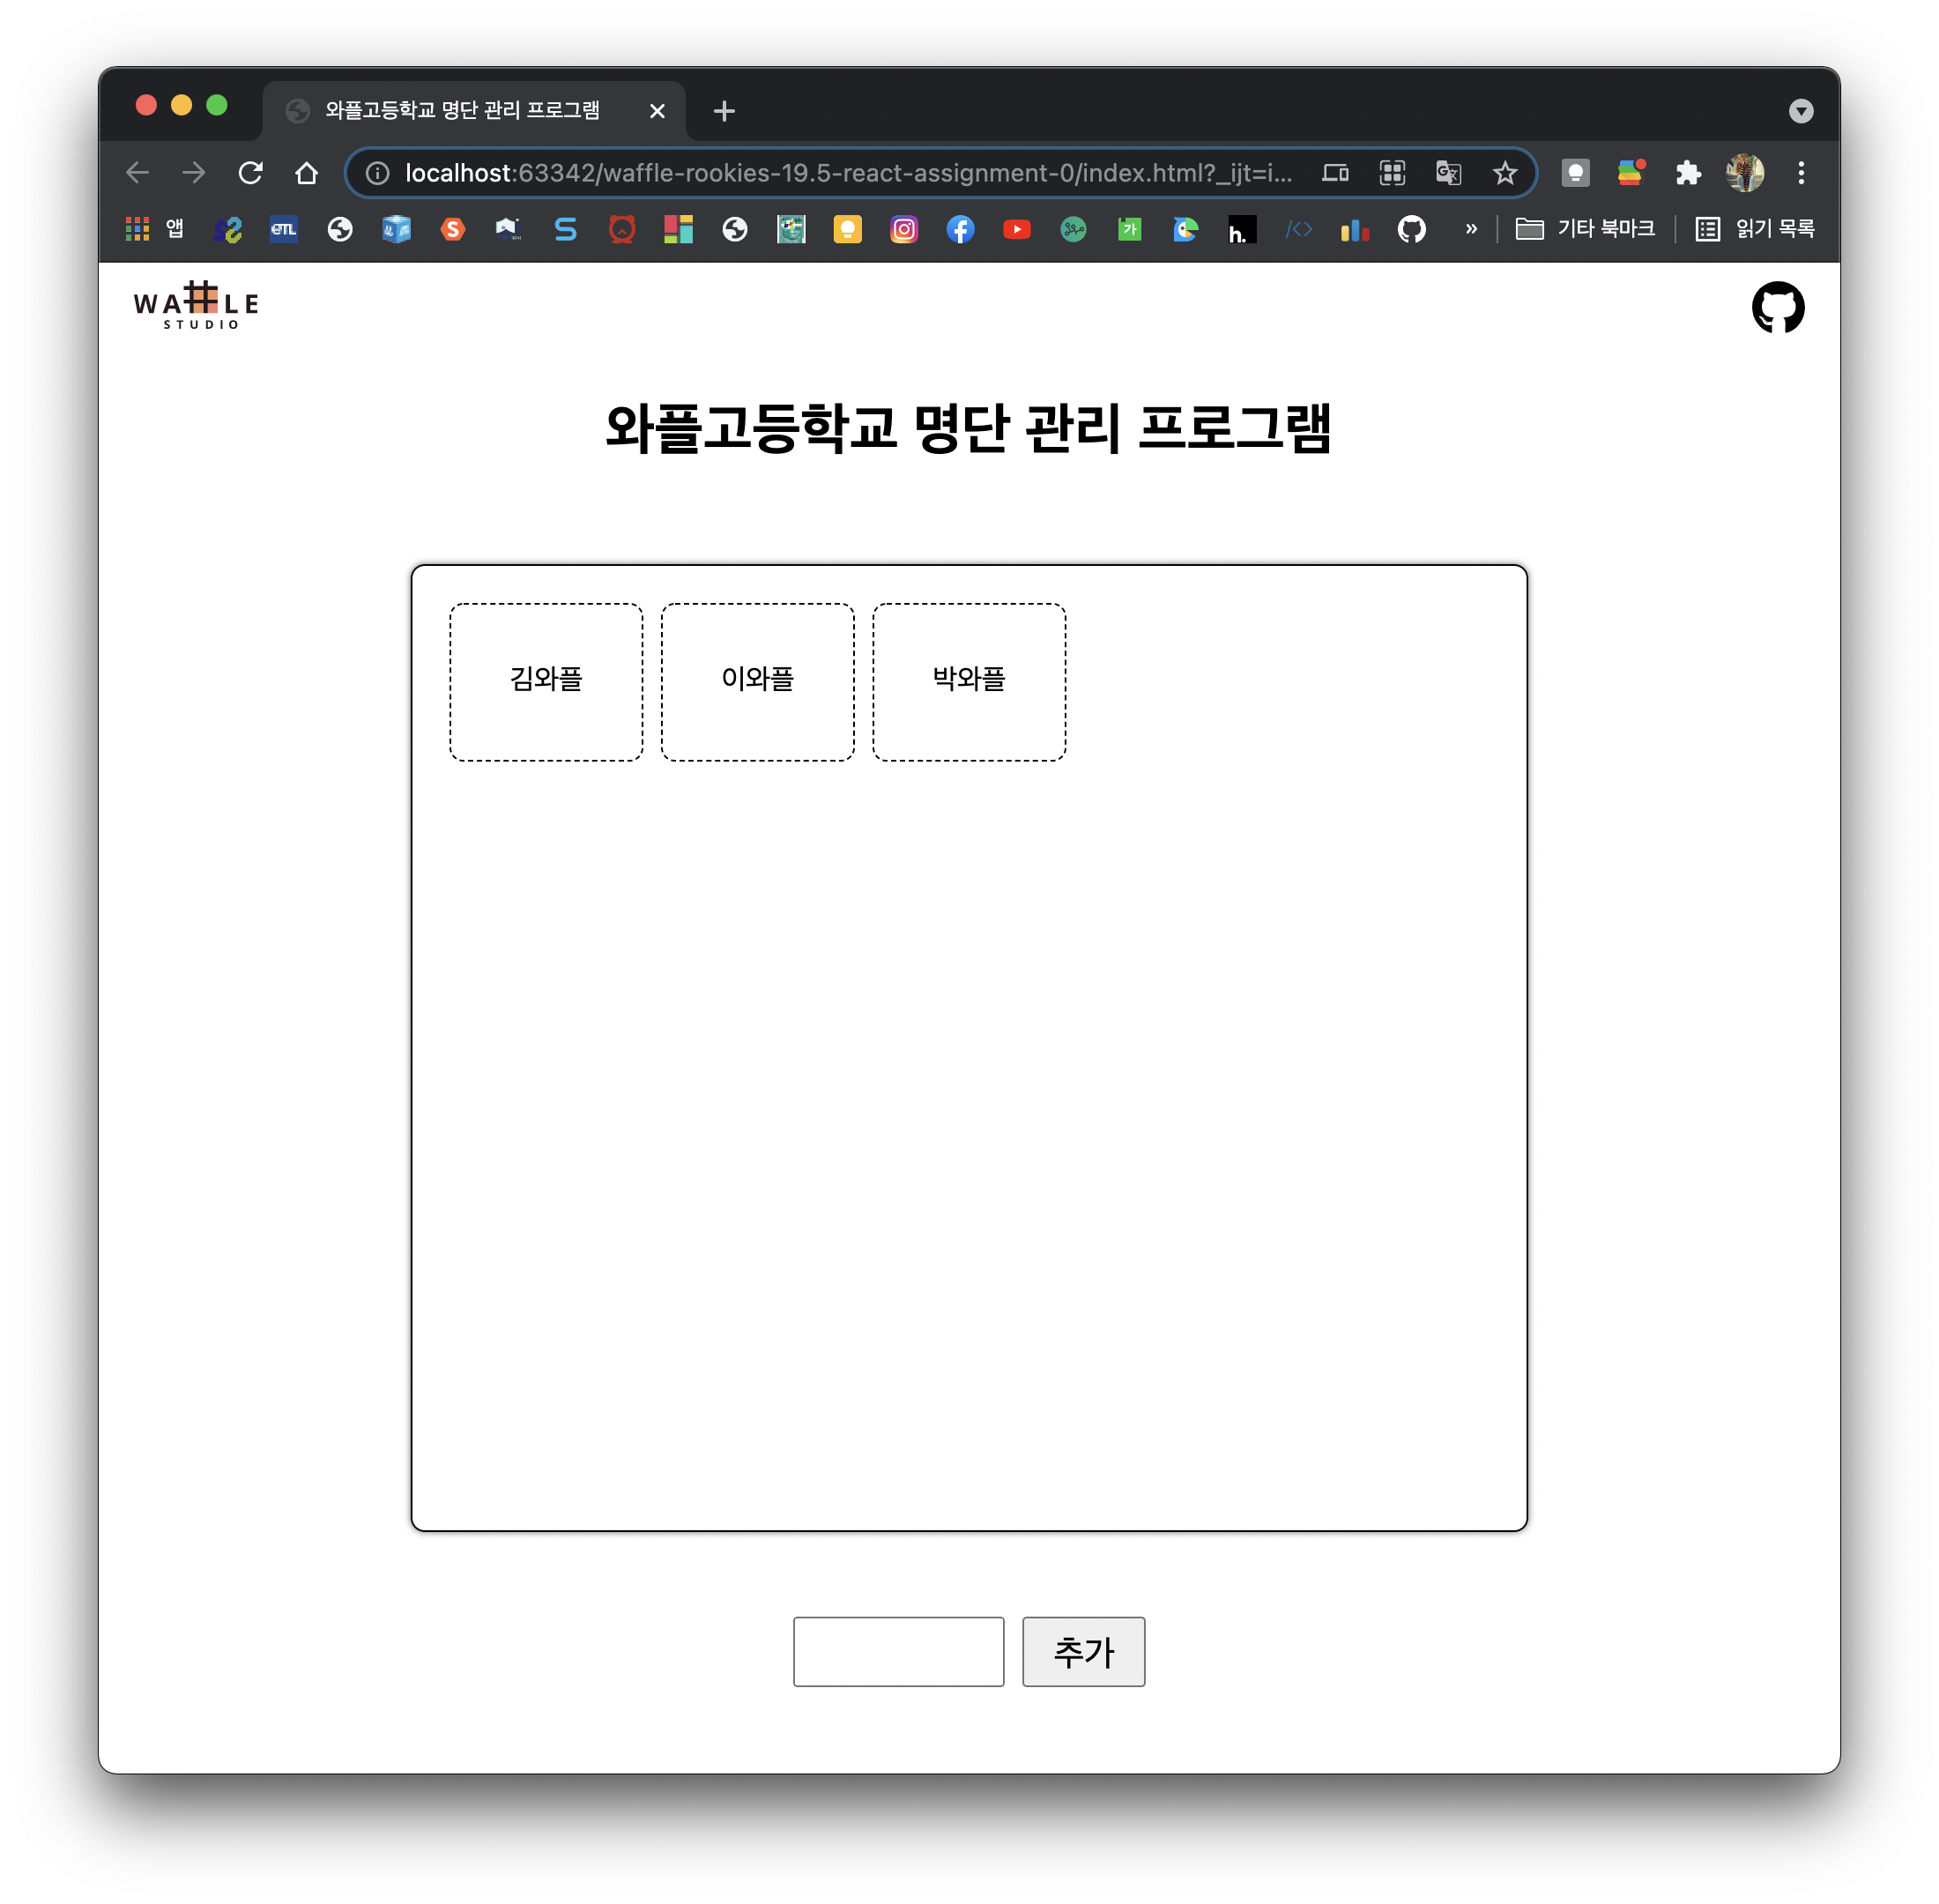
\includegraphics[width=0.19\textwidth]{../images/simulation/1.png}}} \hspace*{1mm}
        \subfloat[]{{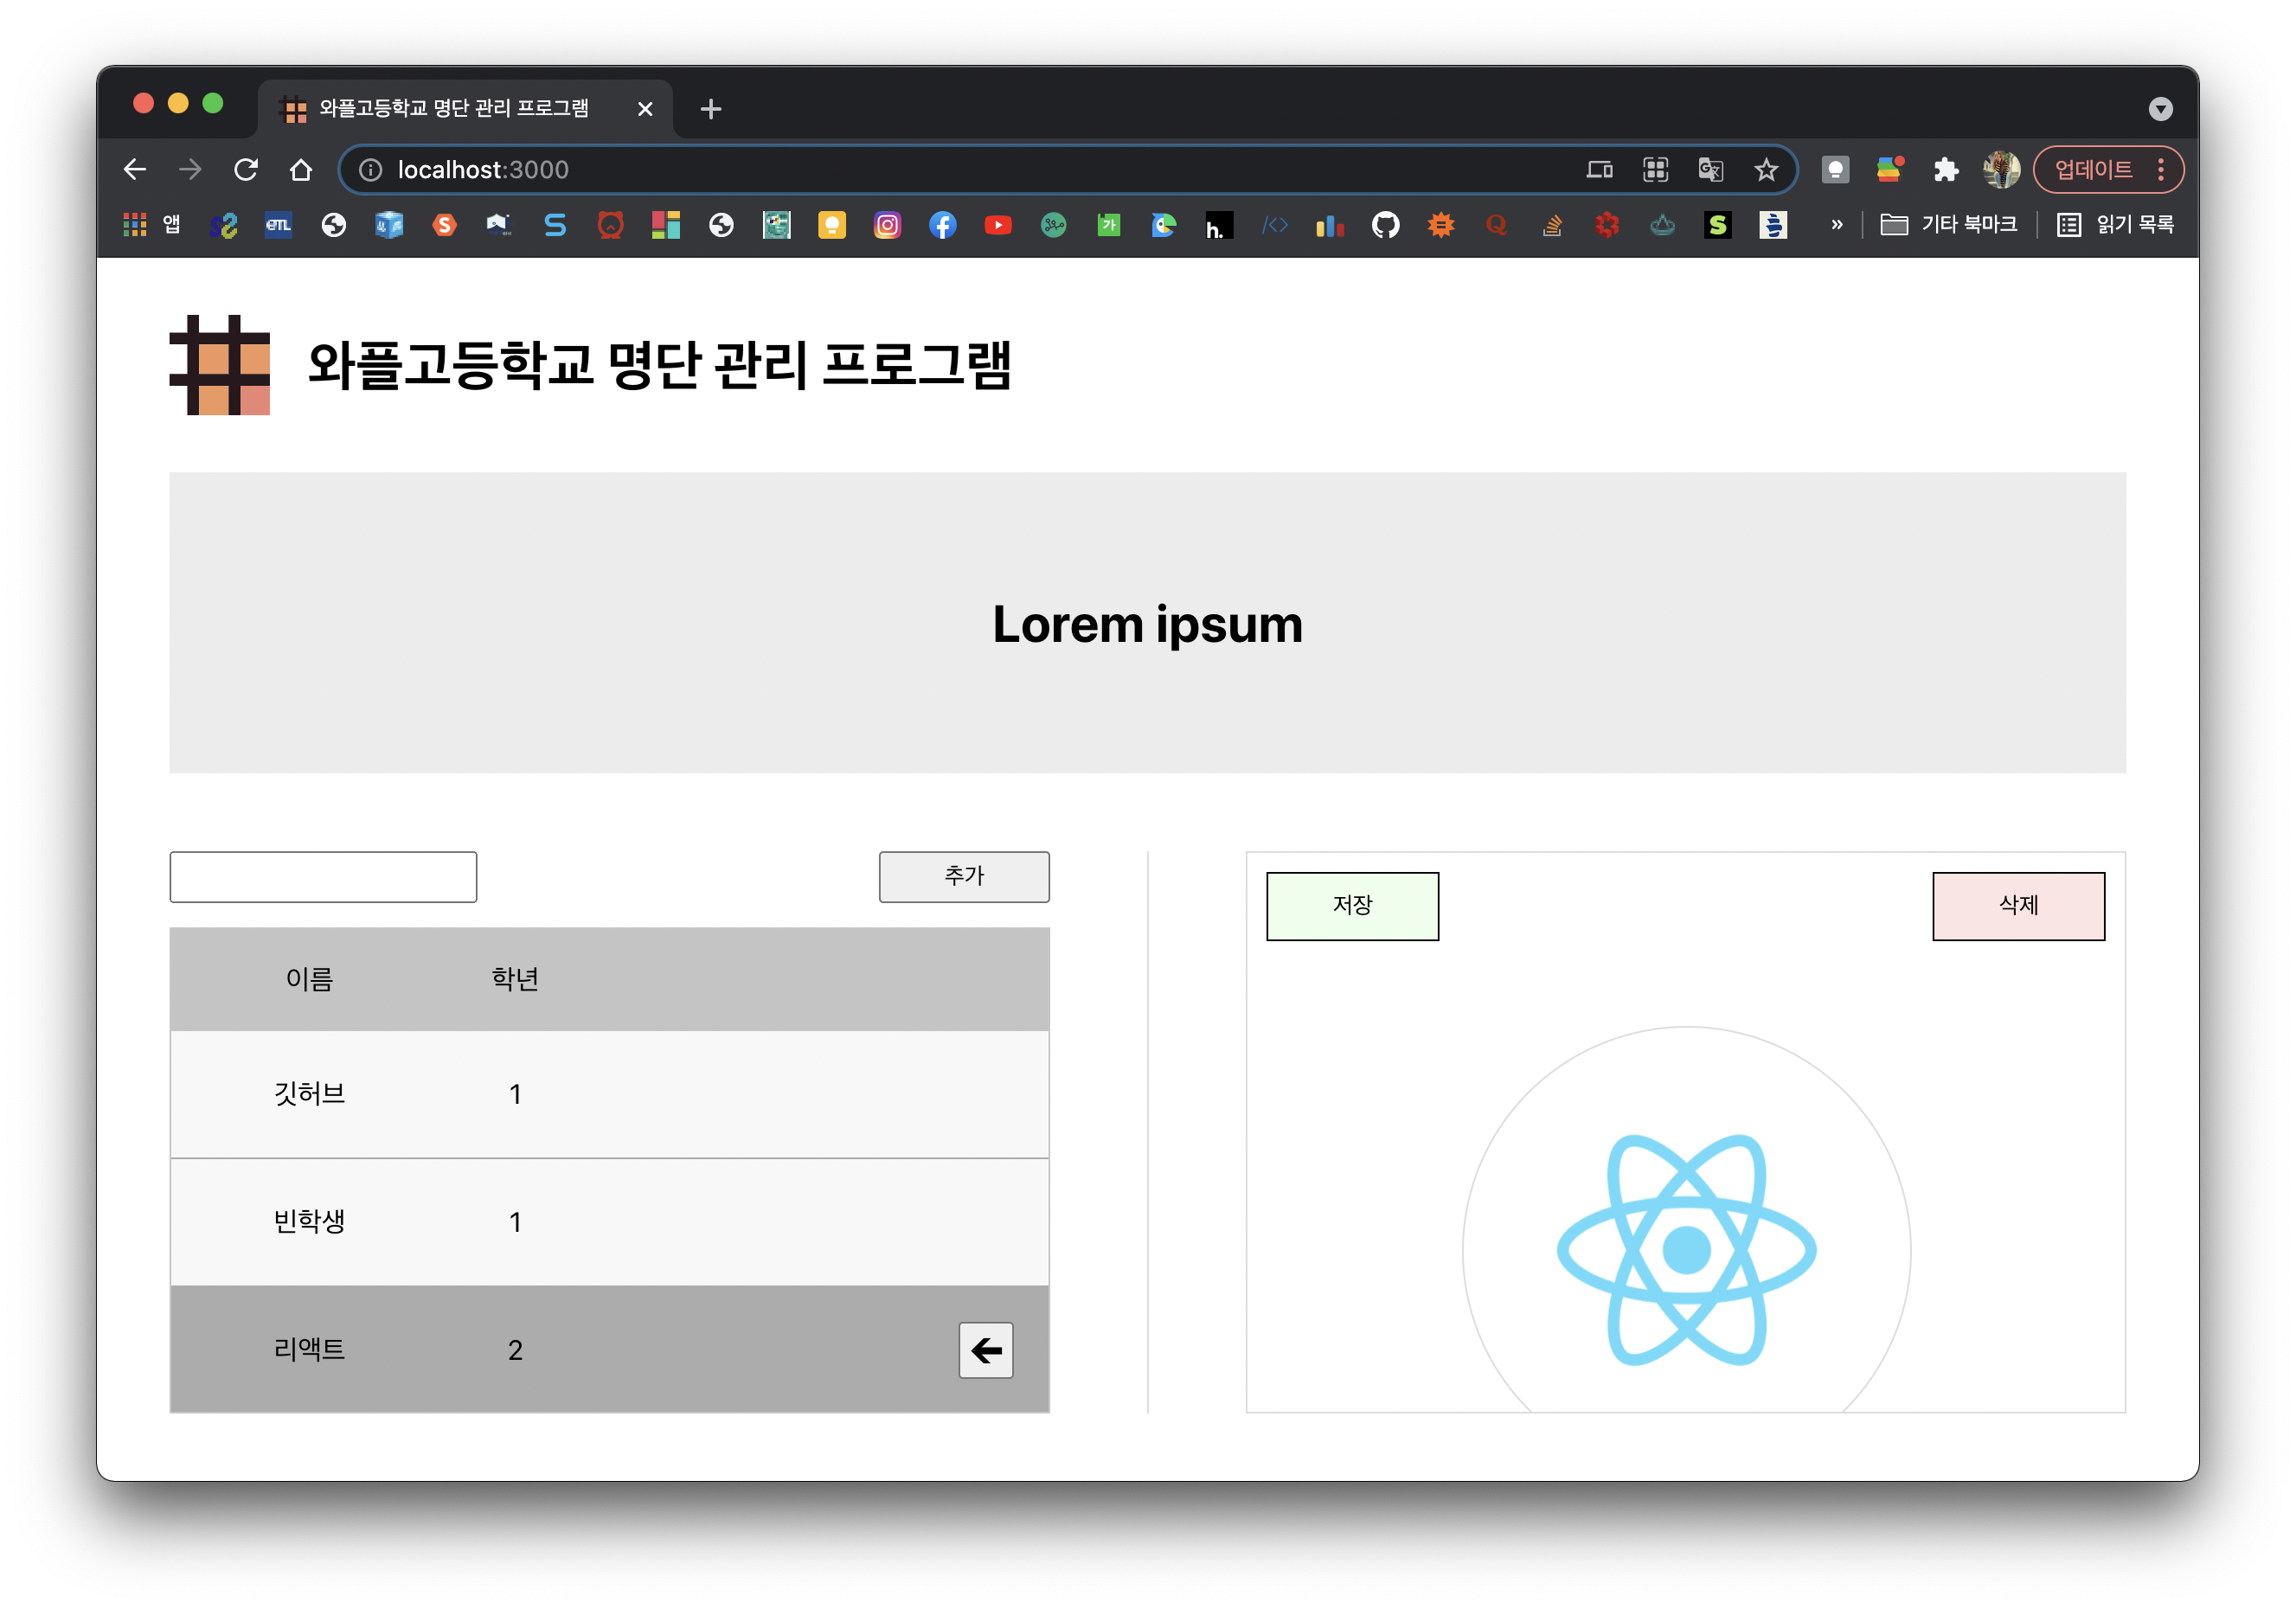
\includegraphics[width=0.19\textwidth]{../images/simulation/3.png}}} \hspace*{1mm}
        \subfloat[]{{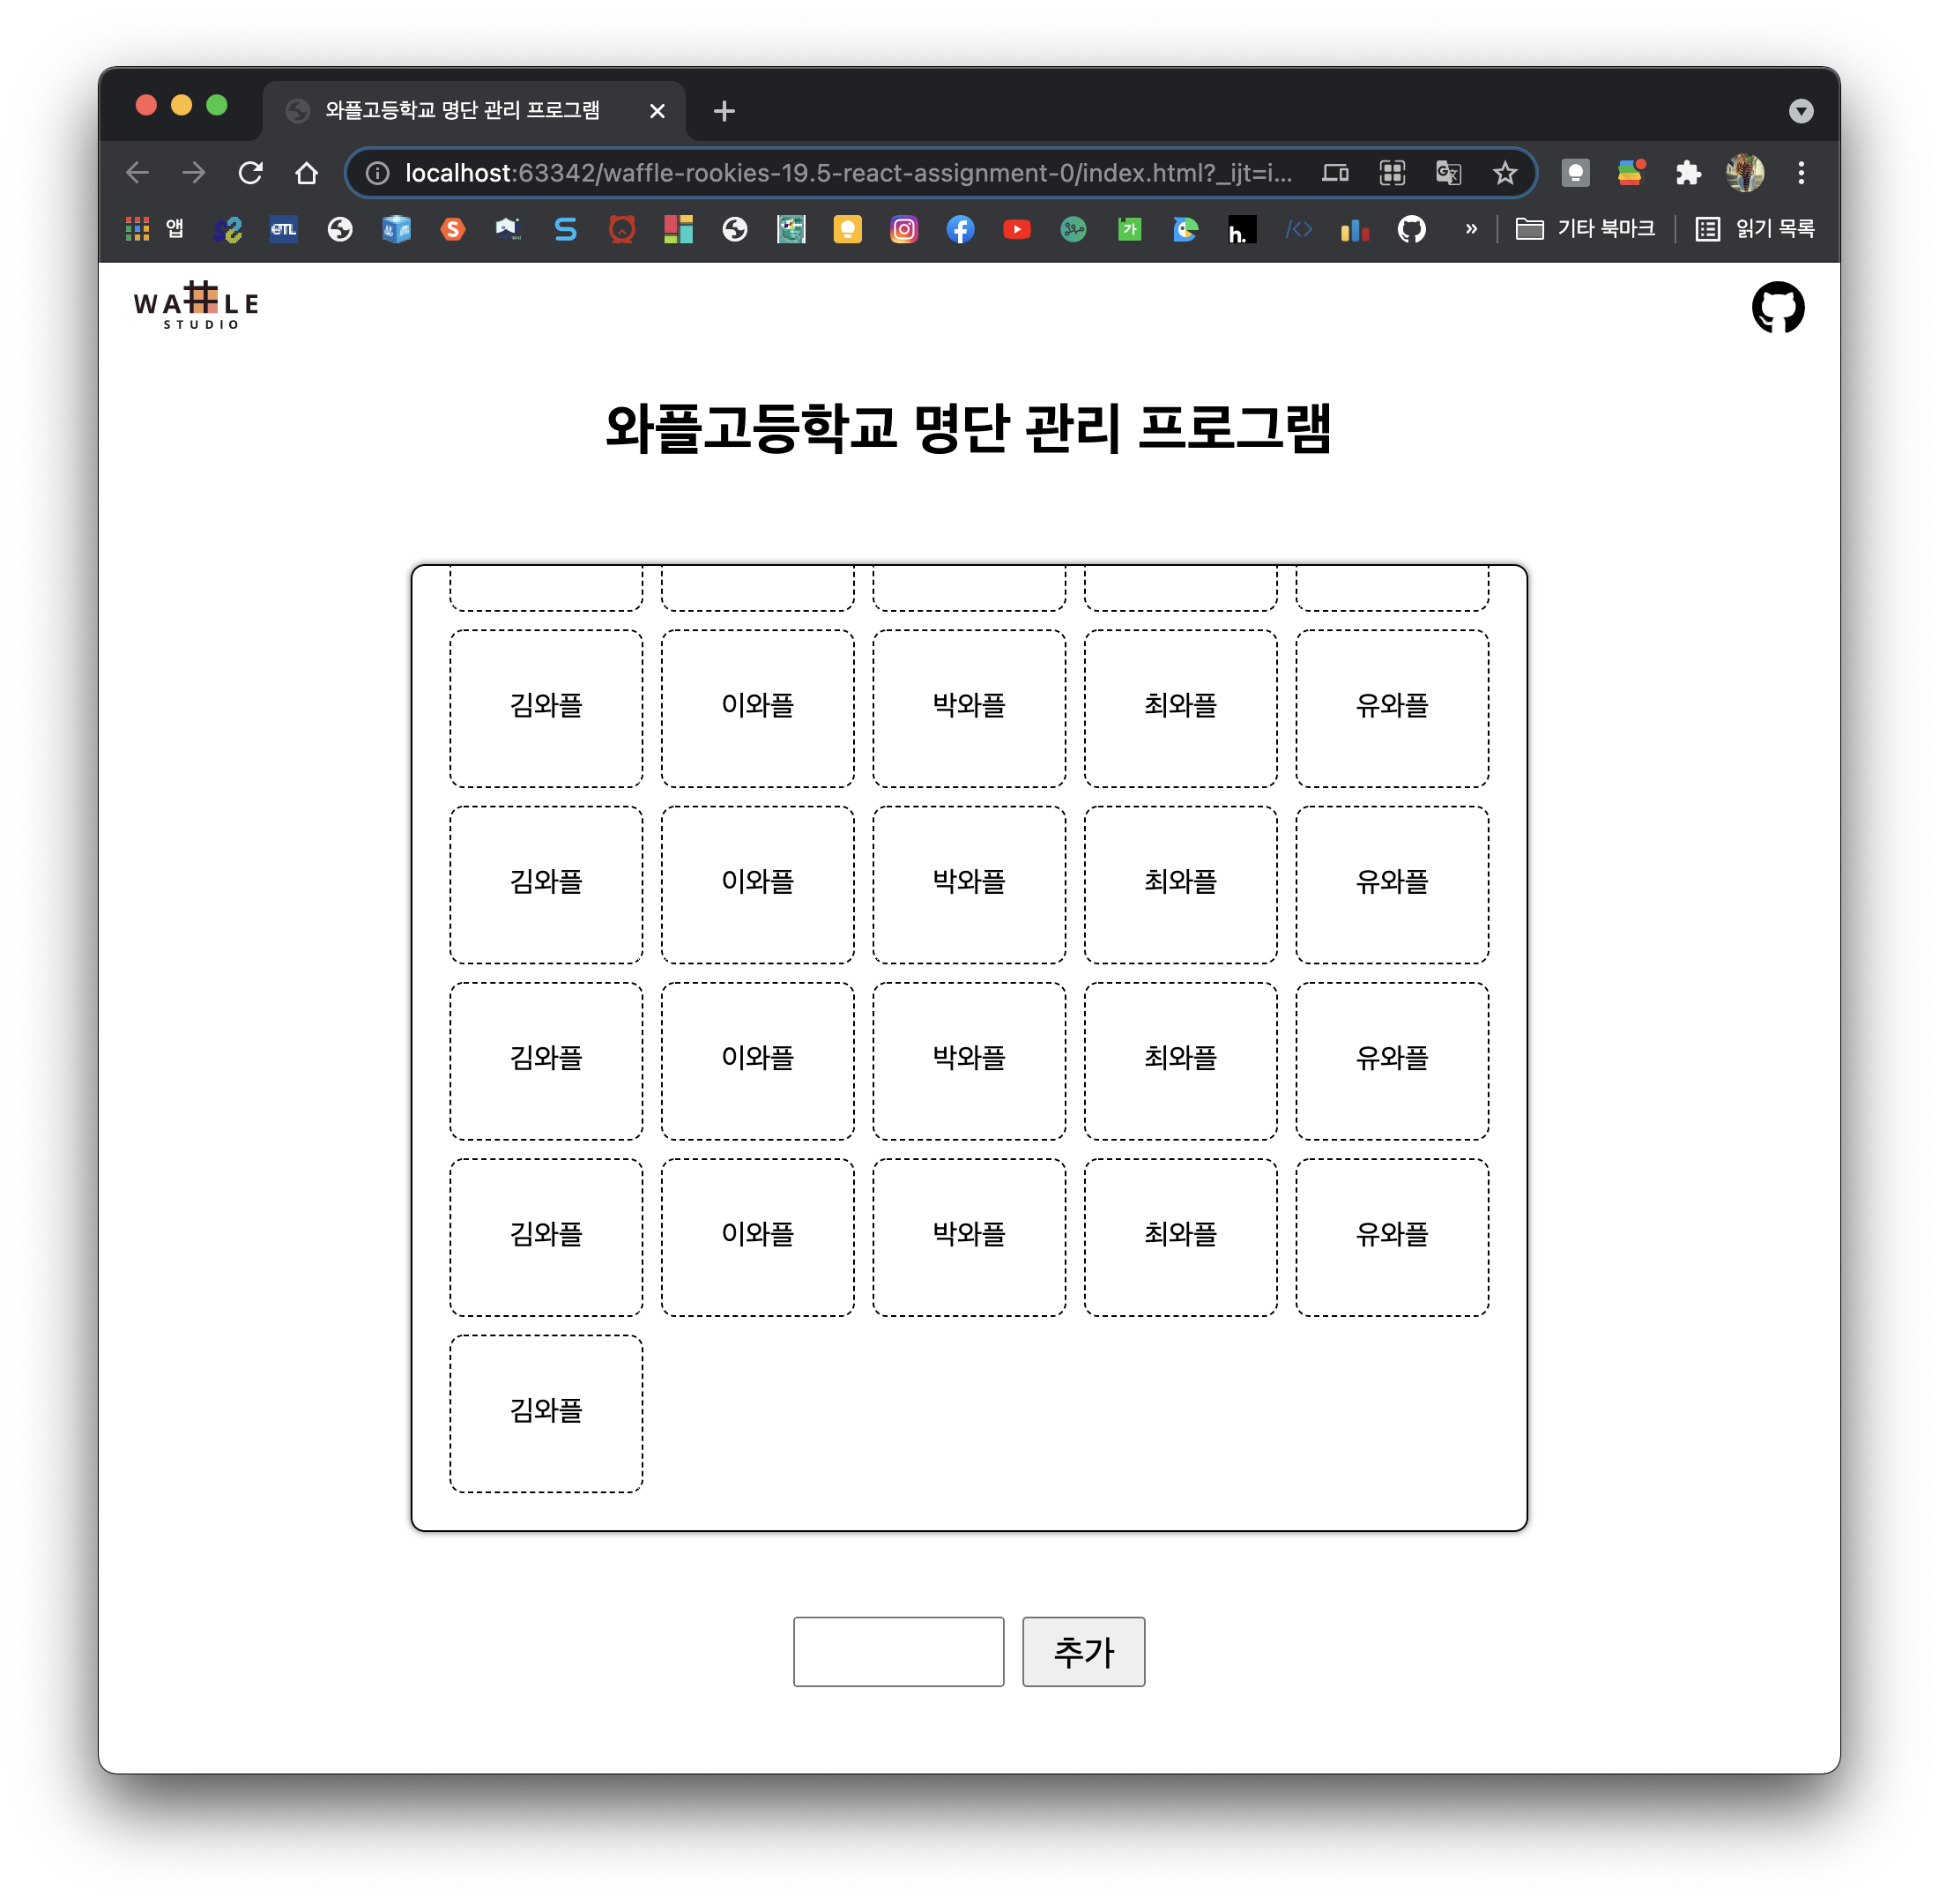
\includegraphics[width=0.19\textwidth]{../images/simulation/4.png}}} \\
        \subfloat[]{{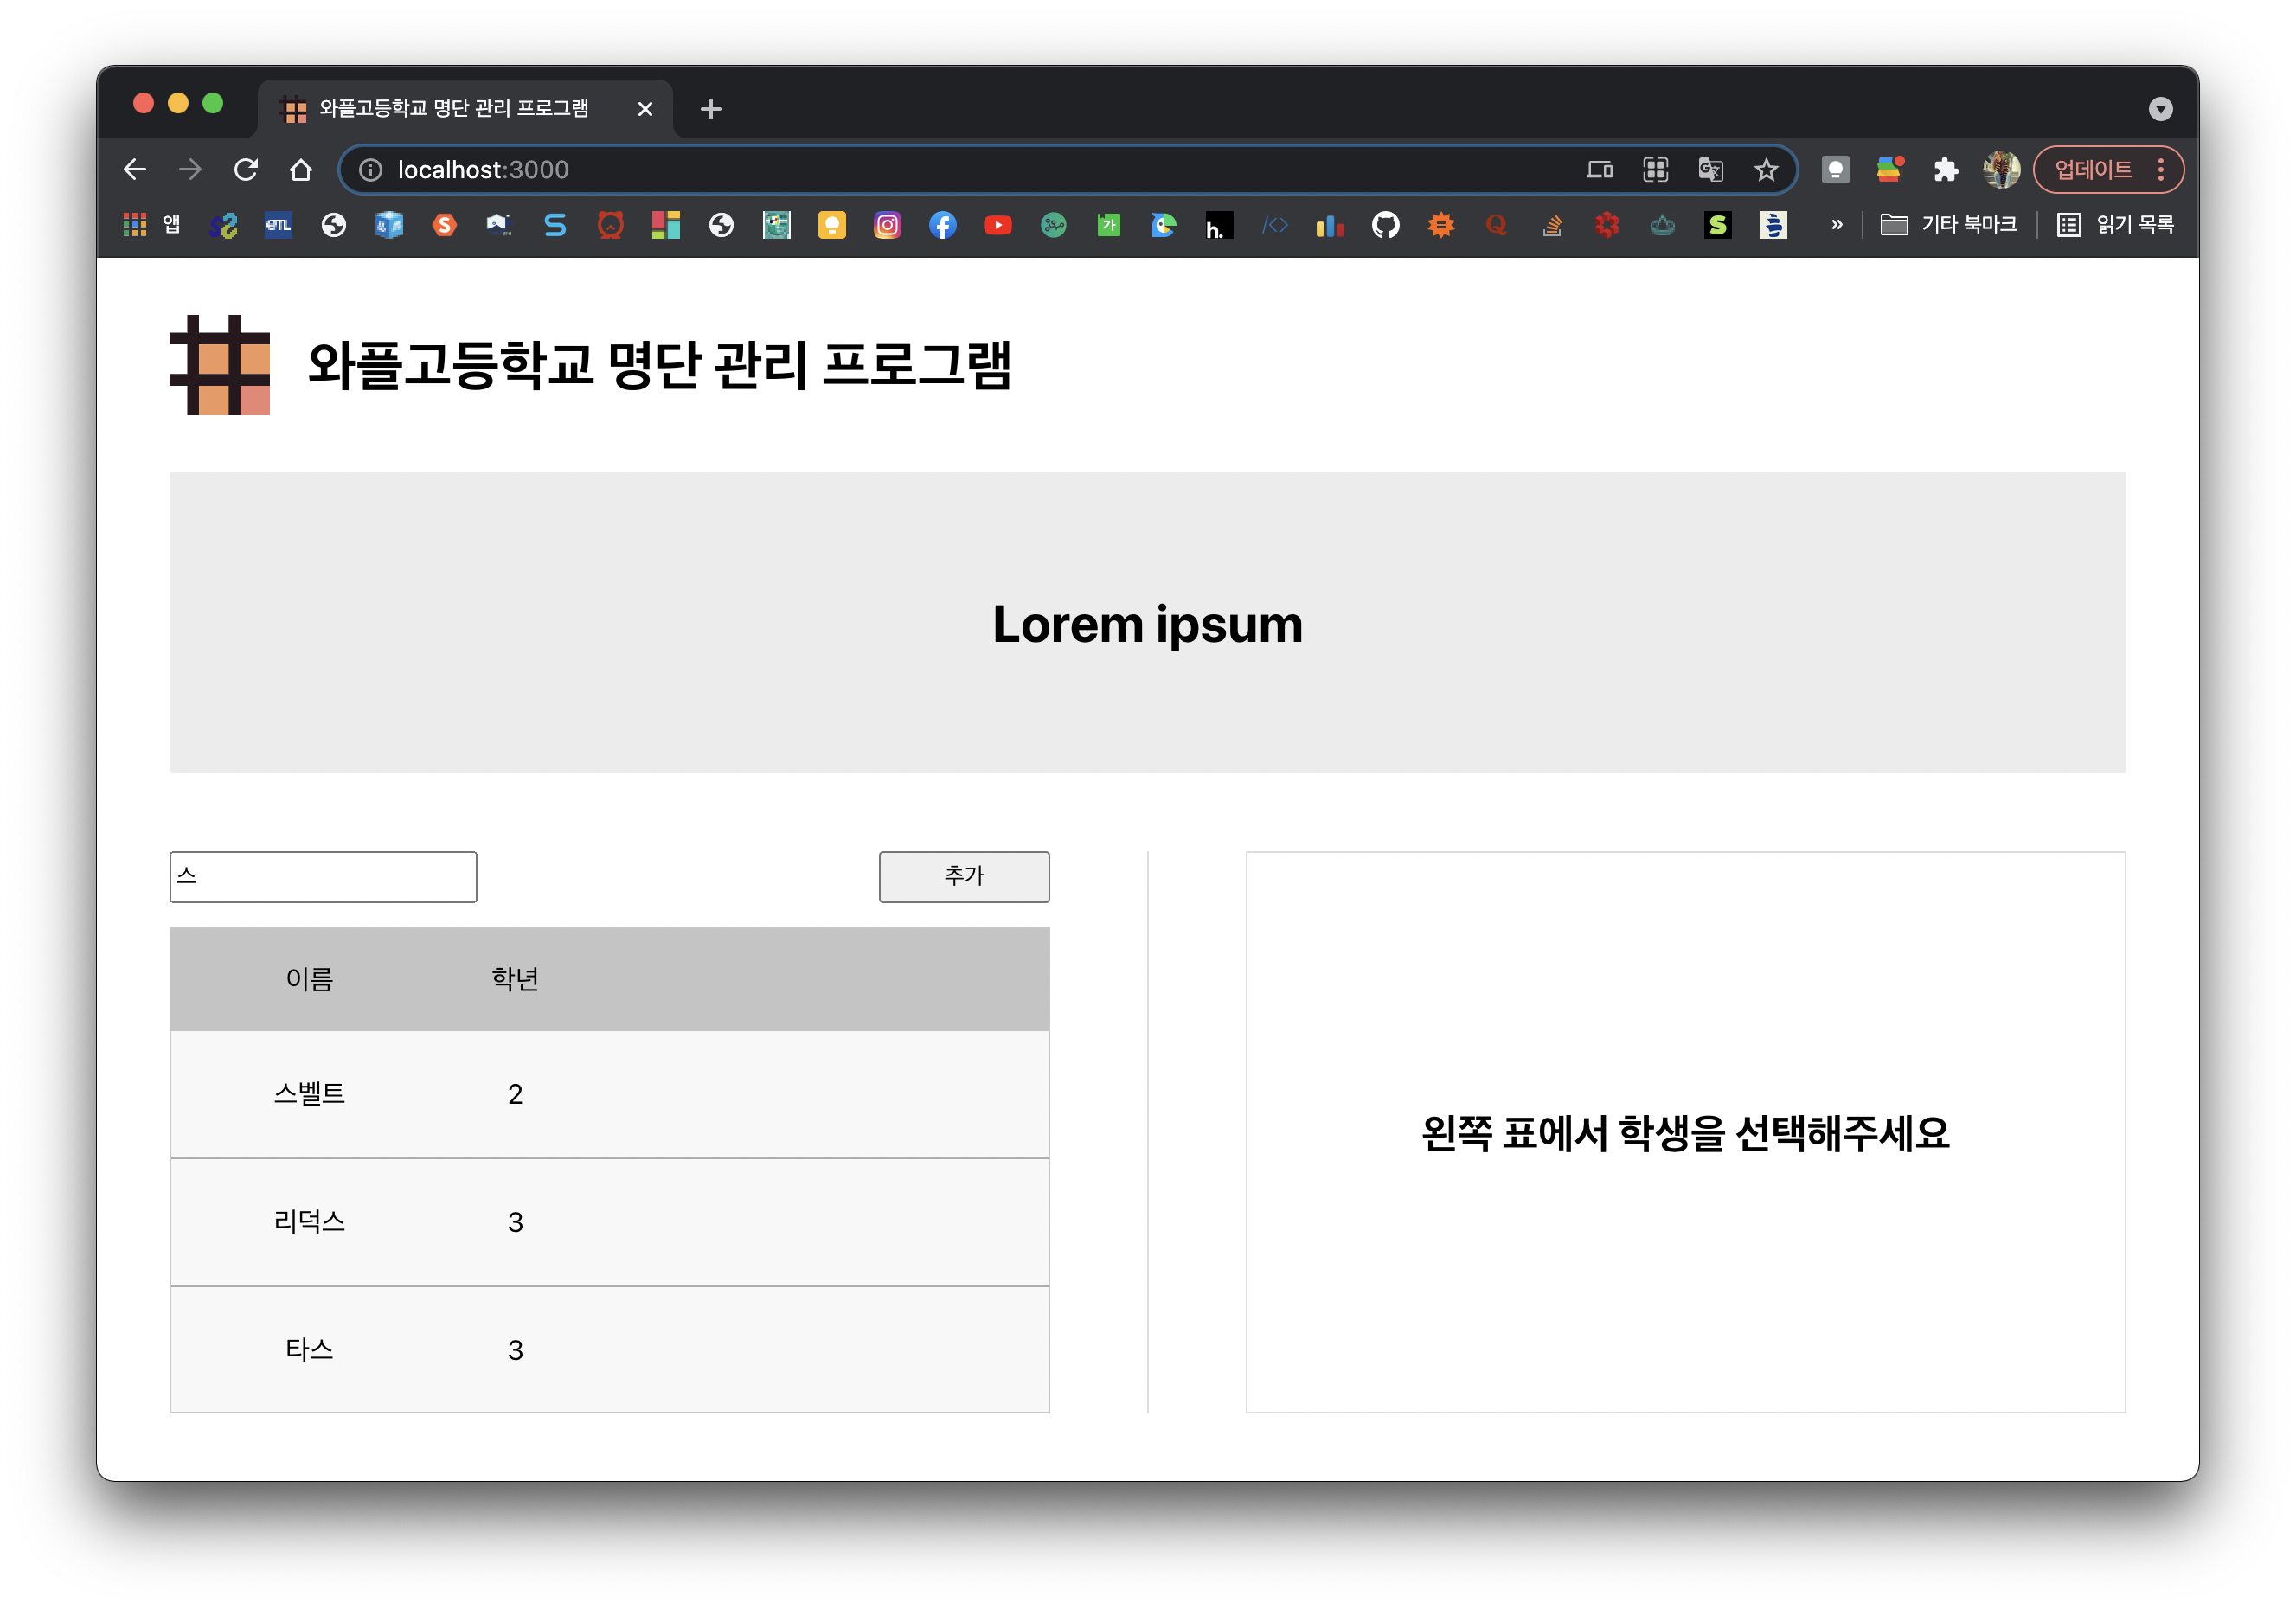
\includegraphics[width=0.19\textwidth]{../images/simulation/5.png}}} \hspace*{1mm}
        \subfloat[]{{\includegraphics[width=0.19\textwidth]{../images/simulation/6.png}}} \hspace*{1mm}
        \subfloat[]{{\includegraphics[width=0.19\textwidth]{../images/simulation/7.png}}} \hspace*{1mm}
        \subfloat[]{{\includegraphics[width=0.19\textwidth]{../images/simulation/8.png}}} \\
        \subfloat[]{{\includegraphics[width=0.19\textwidth]{../images/simulation/9.png}}} \hspace*{1mm}
        \subfloat[]{{\includegraphics[width=0.19\textwidth]{../images/simulation/10.png}}} \hspace*{1mm}
        \subfloat[]{{\includegraphics[width=0.19\textwidth]{../images/simulation/11.png}}} \hspace*{1mm}
        \subfloat[]{{\includegraphics[width=0.19\textwidth]{../images/simulation/12.png}}} \hspace*{1mm}
        \subfloat[]{{\includegraphics[width=0.19\textwidth]{../images/simulation/13.png}}} \hspace*{1mm}
        \caption{\small Microprocessor 테스트 결과. (a)부터 (m)까지 순서대로 진행한 모습이다.}
    \end{figure}

    또한 중간 각 wire의 값까지 포함하여 출력하도록 하여 Xilinx로 simulation을 해보았다. 
    이때 편의상 clock frequency는 2.5MHz로 하였고, 2000ns 시점에서 reset을 입력하였다.
    전체적인 결과는 보드에서 실행한 것과 같은 것을 볼 수 있고, 초기화 이후에는 가장 처음과 같이 실행이 이루어지는 모습을 볼 수 있다.
    
    \begin{figure}[H]
        \centering
        \includegraphics[width=0.99\textwidth]{../images/simulation/sim1.png}
        \includegraphics[width=0.99\textwidth]{../images/simulation/sim2.png}
        \caption{\small Microprocessor 시뮬레이션 결과}
    \end{figure}
\end{document}